\subsection{Soron belüli jelölések}

%23
\begin{frame}
  A soron belüli formázó elemek közül előnyben részesítjük azok használatát, melyek \emph{szemantikai többletet}
  adnak a szöveg tartalmának, a pusztán \emph{formázási célú} elemekkel szemben $\to$ erre ott a CSS!
  \vfill
  Ettől függetlenül, néhány, csak formázási célú elem használata továbbra is szabványos a HTML5-ben.
  \vfill
  \begin{description}[m]
    \item[\texttt{<small>}] \hfill \\ Kisbetűs szöveg. (A \texttt{<big>} elem a HTML5-ben már nem támogatott.)
    \item[\texttt{<i>}] (italics) \hfill \\ Döntötten szedett szöveg, jelentéstöbblet nélkül.
    \item[\texttt{<em>}] (emphasized) \hfill \\ Hangsúlyos, fontos szövegrész, melyet a böngésző alapértelmezetten általában dőlt betűkkel jelenít meg.
  \end{description}
\end{frame}

%24
\begin{frame}
  \begin{description}[m]
    \small
    \item[\texttt{<b>}] (bold) \hfill \\ Félkövéren szedett szöveg, jelentéstöbblet nélkül.
    \item[\texttt{<strong>}] (strong importance) \hfill \\ Kiemelten hangsúlyos, fontos szövegrész, melyet a böngésző alapértelmezetten általában félkövér betűkkel jelenít meg.
    \item[\texttt{<sup>}] (superscript) \hfill \\ Felső index.
    \item[\texttt{<sub>}] (subscript) \hfill \\ Alsó index.
    \item[\texttt{<ins>}] (inserted) \hfill \\ Utólag beszúrt szöveg (ált. aláhúzással jelölve).
    \item[\texttt{<del>}] (deleted) \hfill \\ Kitörölt szöveg (ált. áthúzással jelölve).
    \item[\texttt{<mark>}] \hfill \\ Kijelölt szöveg (ált. sárga háttérrel kiemelve).
  \end{description}
\end{frame}

%25
\begin{frame}
  \begin{columns}[c]
    \column{0.7\textwidth}
      Próbálja meg előállítani azt a HTML fájlt, ami a jobb oldalon látható módon jelenik meg a böngészőben!
      Kiinduláshoz felhasználhatja a dokumentum \textattachfile{soronbelul.txt}{nyers szövegét}.
      Ne feledje, hogy az olyan, önmagukban is jelentéssel bíró karakterek megjelenítése, mint pl. a \kiemel{<}
      karakter, \hiv{\href{https://en.wikipedia.org/wiki/List_of_XML_and_HTML_character_entity_references\#Character_entity_references_in_HTML}{HTML entitásokkal}} lehetséges.
    \column{0.3\textwidth}
      \begin{center}
        \begin{exampleblock}{\textattachfile{soronbelul.html}{soronbelul.html}}
          \centering 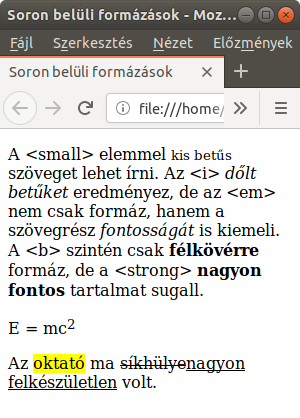
\includegraphics[scale=.35]{soronbelul.png}
        \end{exampleblock}
      \end{center}
  \end{columns}
\end{frame}
